\documentclass[conference,a4paper]{IEEEtran}
\IEEEoverridecommandlockouts
% The preceding line is only needed to identify funding in the first footnote. If that is unneeded, please comment it out.
\usepackage{cite}
\usepackage{amsmath,amssymb,amsfonts}
\usepackage{algorithmic}
\usepackage{graphicx}
\usepackage{textcomp}
\usepackage{xcolor}
\usepackage{url} % line breaking for URLs in the bibliography
\graphicspath{{figures/}}
\def\BibTeX{{\rm B\kern-.05em{\sc i\kern-.025em b}\kern-.08em
    T\kern-.1667em\lower.7ex\hbox{E}\kern-.125emX}}

% Task/section placeholders: everything in red is unfinished prose.
\newcommand{\todo}[1]{\textcolor{red}{[TODO: #1]}}

\begin{document}

\title{Safe Human--Robot Collaborative Assembly via Learning from Demonstration and Variable Impedance Control}

\author{\IEEEauthorblockN{Member A, Member B, Member C, Member D, and Member E}
\IEEEauthorblockA{\textit{Placeholder Affiliation} \\
Placeholder Department, Placeholder University\\
Placeholder City, Placeholder Country}}

\maketitle

\begin{abstract}
% Owner: A | Page budget: 0.75 pages (Abstract + Sec. I combined)
\todo{Summarize the safe box-in-box assembly problem, the GMM/GMR learning and variable impedance pipeline, the MuJoCo/Franka evaluation and the headline quantitative results in 150--200 words.}

\end{abstract}

% Owner: A | Page budget: 0.75 pages (Abstract + Sec. I combined)
\section{Introduction}
\label{sec:intro}
\todo{Motivate safe human--robot collaborative assembly, state the gap between stiff position control and compliant contact tasks, and list the four contributions (system model, LfD pipeline, variable impedance law, ISO/TS 15066 evaluation).}

% Owner: A | Page budget: 0.75 pages
\section{Related Work}
\label{sec:related}
\todo{Review impedance and operational-space control \cite{hogan1985impedance,khatib1987unified}, learning from demonstration \cite{calinon2007learning,kana2023boxinbox}, variable impedance and tank-based passivity \cite{ferraguti2013tank}, and robot safety standards \cite{iso15066,iso10218,haddadin2017collision}.}

% Owner: B | Page budget: 1.0 pages
\section{Requirements and System Architecture}
\label{sec:requirements}
\todo{Derive the functional and safety requirements for collaborative box-in-box assembly (accuracy, contact force, cycle time, ISO/TS 15066 limits) and map each one onto a module of the perception--learning--control--monitoring architecture.}

% Owner: C, D, E (IV-A, IV-B, IV-C) | Page budget: 2.0 pages (0.6 + 0.7 + 0.7)
\section{Method}
\label{sec:method}
\todo{Give the one-paragraph overview of the pipeline (demonstration $\rightarrow$ GMM/GMR reference $\rightarrow$ variable impedance tracking $\rightarrow$ safety monitor) and forward the details to Sections~\ref{sec:modeling}--\ref{sec:vic}.}

% Owner: C | Page budget: 0.6 pages
% Limits: <=1.25 column, <=350 words, <=5 equations, <=1 figure + 1 table
\subsection{System Modeling}
\label{sec:modeling}

We model a box-in-box cell inspired by~\cite{kana2023boxinbox} in MuJoCo~\cite{todorov2012mujoco} ($1\text{ ms}$ step) with a 7-DoF torque-controlled Franka Panda~\cite{menagerie2022,frankadocs} (Fig.~\ref{fig:scene}). A rigid $30\times 30\times 60\text{ mm}$ peg ($0.2\text{ kg}$) is mounted on the flange behind a wrist force/torque (F/T) sensor and inserted into a fixed $40\text{ mm}$-deep square hole ($0.5\text{ mm}$ per-side clearance; $3\text{ mm}$, $45^\circ$ chamfer). All quantities are in SI units. The world frame $\{W\}$ is at the robot base ($z$ up) and the tool-centre-point (TCP) frame $\{T\}$ is at the peg end-face centre. For joint positions $q \in \mathbb{R}^7$, forward kinematics (FK) gives the TCP pose $x$ from the modified DH chain~\cite{frankadocs,menagerie2022}, and $J(q) \in \mathbb{R}^{6\times 7}$ maps $\dot{q}$ to the TCP twist $\dot{x}$ (linear $v$, angular $\omega$) in $\{W\}$:
\begin{equation}
\dot{x} = [v;\,\omega] = J(q)\dot{q}.
\label{eq:twist}
\end{equation}

\begin{figure}[t]
\centering
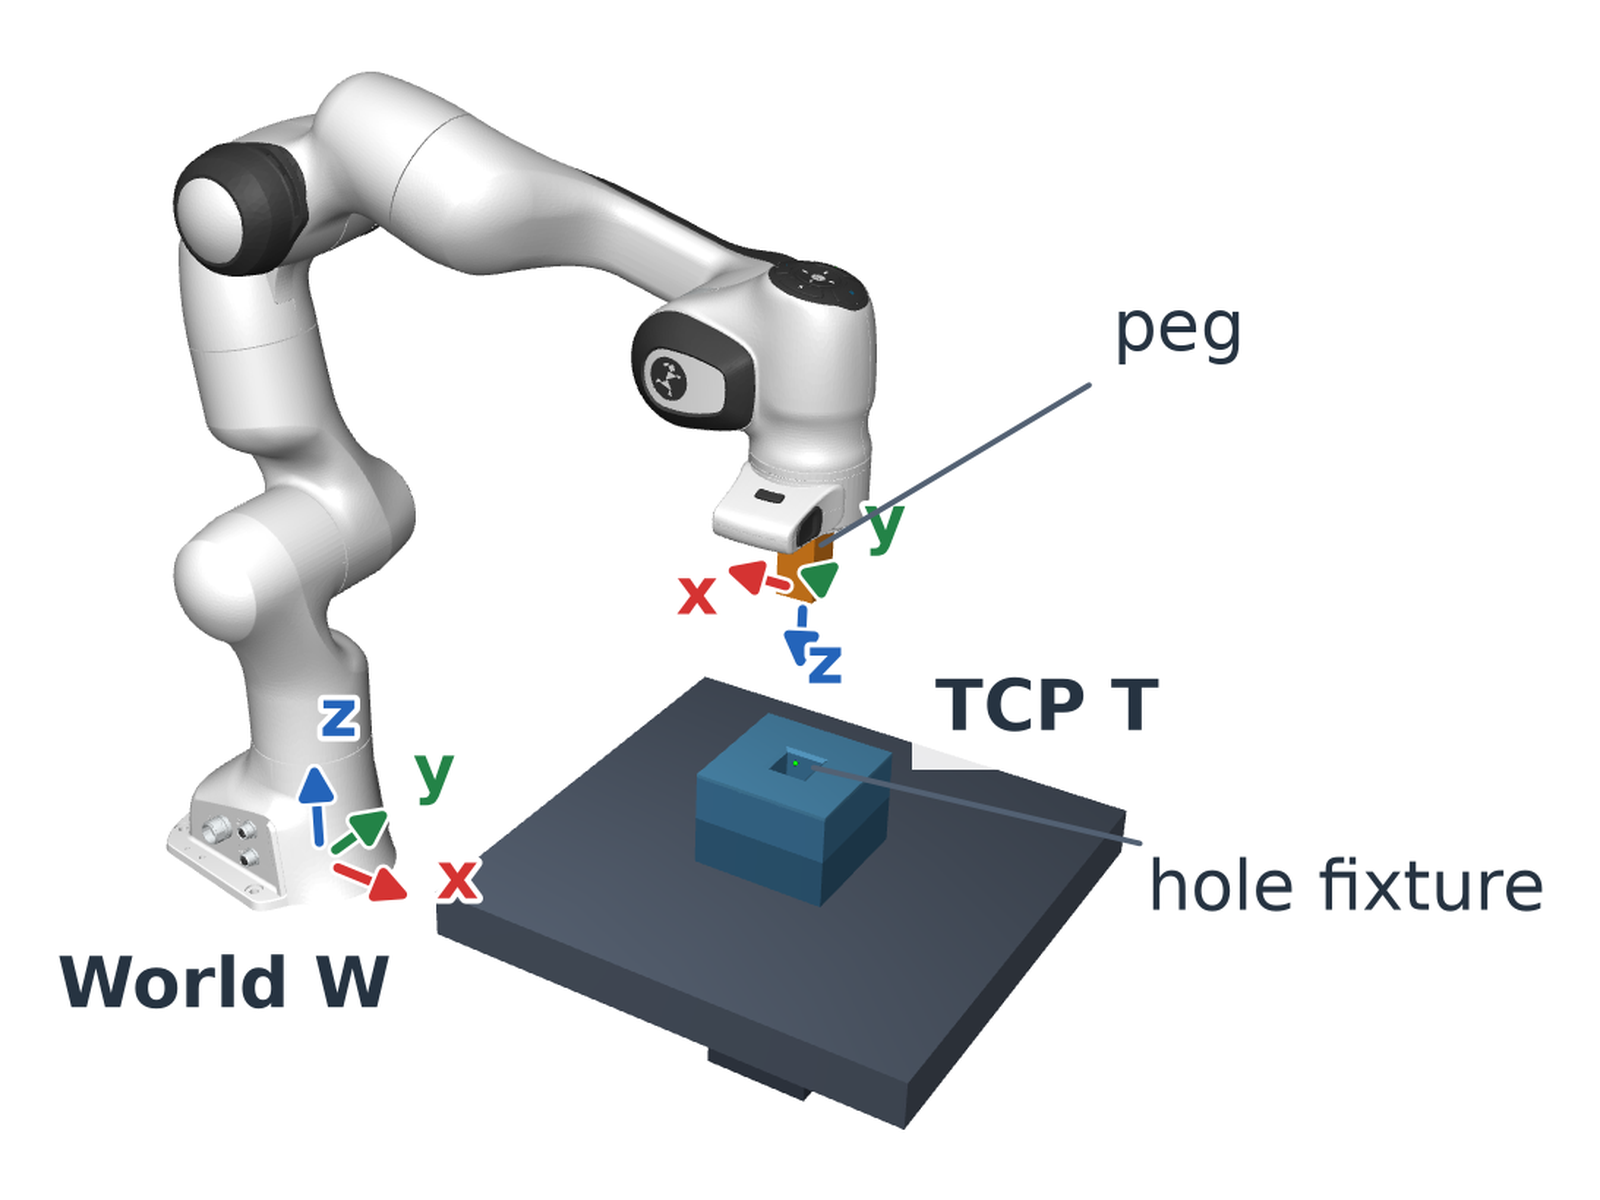
\includegraphics[width=0.6\columnwidth]{scene.png}
\caption{Simulated box-in-box setup with frames $\{W\}$ and $\{T\}$.}
\label{fig:scene}
\end{figure}

With rigid-body inertia $M_{rb}(q)$, armature $I_a = 0.1 I_7\text{ kg}\cdot\text{m}^2$, total inertia $\mathcal{M}(q) = M_{rb}(q) + I_a$, Coriolis term $h(q,\dot{q}) = C(q,\dot{q})\dot{q}$, gravity $g(q)$, viscous damping $D = 1.0 I_7\text{ N}\cdot\text{m}\cdot\text{s/rad}$, and external joint torque $\tau_{\text{ext}}$ ($= J^T F_{\text{ext}}$ for a wrench $F_{\text{ext}} \in \mathbb{R}^6$ applied by the environment at the TCP):
\begin{equation}
(M_{rb}(q) + I_a)\ddot{q} + C(q,\dot{q})\dot{q} + g(q) + D\dot{q} = \tau + \tau_{\text{ext}}.
\label{eq:joint_eom}
\end{equation}
The motor torque is the controller torque $\tau_{\text{cmd}}$ plus gravity compensation, saturated at the joint torque limits $\tau_{\max}$~\cite{frankadocs}: $\tau = \operatorname{clip}(\tau_{\text{cmd}} + g(q), -\tau_{\max}, +\tau_{\max})$. For task wrench $F \in \mathbb{R}^6$, null-space torque $\tau_0 \in \mathbb{R}^7$, $\ddot{x} = J\ddot{q} + \dot{J}\dot{q}$, and $\tau_{\text{cmd}} = J^T F + N_\tau \tau_0$, the operational-space dynamics~\cite{khatib1987unified} are
\begin{equation}
\Lambda\ddot{x} + \mu = F + F_{\text{ext}}, \qquad \mu = \mu_{rb} + \mu_D,
\label{eq:op_eom}
\end{equation}
with $A = J\mathcal{M}^{-1}J^T$, inertia $\Lambda$, dynamically consistent inverse $\bar{J}$ ($F_{\text{ext}} = \bar{J}^T \tau_{\text{ext}}$), and null-space torque projector $N_\tau$:
\begin{equation}
\Lambda = A^{-1}, \qquad \bar{J} = \mathcal{M}^{-1}J^T\Lambda, \qquad N_\tau = I_7 - J^T\bar{J}^T,
\label{eq:op_proj}
\end{equation}
where $\mu_{rb} = \Lambda(J\mathcal{M}^{-1}h - \dot{J}\dot{q})$, $\mu_D = \Lambda J\mathcal{M}^{-1}D\dot{q}$, and $A$ is regularized as $A + \lambda^2 I_6$ ($\lambda = 0.01$) for robustness near singularities.

The wrist F/T sensor gives $F_{\text{ext}}$ at $\{T\}$ in $\{W\}$ after tool gravity/inertia compensation. The simulator also provides the external joint torque $\tau_{\text{ext}}$, summed over all robot contacts through their contact Jacobians. Contacts use MuJoCo's soft-contact model (friction $0.3$) and a free $0.6\text{ kg}$ hand body whose contact is calibrated so that its impact peak force matches the ISO/TS~15066 hand model ($75\text{ N/mm}$) within $2\%$~\cite{iso15066} (Section~\ref{sec:safety}). Independent NumPy FK, $J$, $\mathcal{M}$, and $g$ match MuJoCo to machine precision (Table~\ref{tab:verification}). With $\lambda = 0$,~\eqref{eq:op_eom}--\eqref{eq:op_proj} reproduce simulated TCP accelerations over $1000$ well-conditioned random states within $2.92\times 10^{-12}\text{ m/s}^2\text{ (or rad/s}^2\text{)}$.

\begin{table}[t]
\centering
\caption{Model verification against MuJoCo and finite differences (max error over 1000 random states)}
\label{tab:verification}
% Generated: six data rows; scoped footnotesize for 252 pt IEEE columns.
{\footnotesize
\setlength{\tabcolsep}{2pt}
\begin{tabular}{@{}lll@{}}
\hline
Quantity & Reference & Max error \\
\hline
TCP pos. [m] & MuJoCo & $1.35\times10^{-15}$ \\
TCP rot. [rad] & MuJoCo & $1.03\times10^{-15}$ \\
$J$ [m/rad; 1] & MuJoCo / FD & $4.11\times10^{-15}$ / $3.40\times10^{-10}$ \\
$\mathcal{M}$ [1] & MuJoCo (rel.) & $3.04\times10^{-15}$ \\
$g$ [N m] & MuJoCo & $6.39\times10^{-14}$ \\
EOM [N m] & Fwd. / inv. & $2.63\times10^{-13}$ / $6.39\times10^{-14}$ \\
\hline
\end{tabular}
}

\end{table}

% Owner: D | Page budget: 0.7 pages
\subsection{Learning from Demonstration}
\label{sec:lfd}
\todo{Present the GMM/GMR formulation used to encode the demonstrations, the task-parameterized input features and the reproduction rule that yields the time-varying reference trajectory.}

% Owner: E | Page budget: 0.7 pages
\subsection{Variable Impedance Control}
\label{sec:vic}
\todo{State the variable impedance law, the stiffness/damping adaptation schedule tied to the task phase, and the tank-based passivity guarantee \cite{ferraguti2013tank}.}


% Owner: A | Page budget: 1.0 pages
\section{Safety Analysis and ISO/TS 15066 Compliance}
\label{sec:safety}
\todo{Map the assembly hazards to quasi-static (clamping) and transient (impact) contact cases, derive the admissible force/pressure limits from ISO/TS 15066 and ISO 10218 \cite{iso15066,iso10218,iso10218part2}, and show how the controller gains and the safety monitor keep every case below those limits \cite{haddadin2017collision}.}

% Owner: B (VI-A), D (VI-B), E (VI-C), A (VI-D) | Page budget: 1.75 pages (0.4 + 0.5 + 0.6 + 0.25)
\section{Experiments}
\label{sec:experiments}

\subsection{Setup}
\label{sec:setup}
\todo{Describe the MuJoCo scene, hardware-in-the-loop assumptions, demonstration protocol, number of trials and the metrics used in B--D.}

\subsection{LfD Results}
\label{sec:lfdresults}
\todo{Report trajectory reproduction accuracy, generalization to perturbed box poses and the comparison against the demonstrated reference.}

\subsection{VIC Results}
\label{sec:vicresults}
\todo{Report insertion success rate, contact forces and completion time for fixed- versus variable-impedance control.}

\subsection{Safety Results}
\label{sec:safetyresults}
\todo{Show measured peak contact forces/pressures against the ISO/TS 15066 limits for each contact case.}

% Owner: A | Page budget: 0.4 pages (VII + VIII combined)
\section{Discussion}
\label{sec:discussion}
\todo{Interpret the results, state the limitations of the simulation-only evaluation and the threats to validity, and sketch the transfer to the real cell.}

% Owner: A | Page budget: 0.4 pages (VII + VIII combined)
\section{Conclusion}
\label{sec:conclusion}
\todo{Restate what was shown, the safety case that supports it, and the next steps (real-robot validation, force-torque sensing, multi-box variants).}


% remove when all refs are cited in text
\nocite{*}

\bibliographystyle{IEEEtran}
\bibliography{refs}

\end{document}
